\documentclass[a4paper]{article}

%use the english line for english reports
\usepackage[english]{babel}
%\usepackage[portuguese]{babel}
\usepackage[utf8]{inputenc}
\usepackage{indentfirst}
\usepackage{enumerate}
\usepackage{graphicx}
\usepackage{verbatim}
\usepackage{url}


\begin{document}

\setlength{\textwidth}{16cm}
\setlength{\textheight}{22cm}

\title{\Huge\textbf{Mbrane}\linebreak\linebreak\linebreak
\Large\textbf{Final Report}\linebreak\linebreak
\linebreak\linebreak

\includegraphics[scale=0.1]{feup-logo.png}\linebreak\linebreak
\linebreak\linebreak
\Large{Logic Programing}\linebreak
}

\author{\textbf{Group Mbrane 4:}\\ Leonardo Fernandes Moura - 201706907@fe.up.pt \\ João Pedro Campos - up201704982@fe.up.pt \\\linebreak\linebreak \\
 \\ Faculdade de Engenharia da Universidade do Porto \\ Rua Roberto Frias, s\/n, 4200-465 Porto, Portugal \linebreak\linebreak\linebreak
\linebreak\linebreak\vspace{1cm}}
\date{November 13, 2019}
\maketitle
\thispagestyle{empty}

%************************************************************************************************
%************************************************************************************************

\newpage

\section*{Summary}

The goal of this project was to program a board game using the prolog language. In our case the game in question is Mbrane, a 
game created by DukeZhou based on Sudoku and strategy games like chess. Section 2 clarifies all the aspects of this game.

\paragraph{}
In terms of programing, the goal of the project was to efficiently implement all the game logic using Prolog.  This means we have to
represent the core mechanics of the game using Prolog. The first step is to find a way to represent the game board that's both 
efficient and relatively simple to program and operate. Then our goal is to make the game playable, continuously updating the state of
the board as both players make their moves. In order to termiate the game and find the winner, we need to detect when the board is in a completed 
state, then we calculate the winner and present it. After the game is playable, the final step is to make it possible to play against the computer 
programing a bot that would be able to play in two difficulty settings. The first one (the easy mode) simply makes random plays, the second 
one calculates the best play it can make at the moment (greedy approach). This means we end up with three different game modes: player versus player,
player versus bot and bot versus bot. 

\paragraph{}
Besides all the game logic, the player needs to interact with the game, so we need to develop a simple text base UI, using
Prolog predicates that are able to interact with the terminal input/output stream. This allows us to read inputs from the
player (or both players) so that we can use them make moves.

\paragraph{}
The prolog distribution used was SicStus Prolog using a Student License.

\newpage

\tableofcontents

%************************************************************************************************
%************************************************************************************************

%*************************************************************************************************
%************************************************************************************************

\newpage

%%%%%%%%%%%%%%%%%%%%%%%%%%
\section{Introduction}
\paragraph{}
This project was developed during the Logic Programing Course in the context of the third the Integrated Masters in Informatics 
and Computing Engineering. The goal is to implement in Prolog a board game, in this case \textit{Mbrane}.

%%%%%%%%%%%%%%%%%%%%%%%%%%
\pagebreak
\section{Game Presentation}

\subsection{Origin}

\paragraph{}
Mbrane is a fairly recent game. It was created in 2013 by someone who goes by the name of DukeZhou. 
When he was a kid, DukeZhou really liked to play strategy board games, but he didn’t like games where luck was a 
relevant factor, he liked games where the player with superior strategy or the one “who played better” was definitely the winner. 
Games like chess or checkers were all he was into. n 2005 he discovered Sudoku, and even though puzzles were not his favorite type 
of game, he was amazed by the game. The sheer amount of combinations for a 9x9 board is around $6.7*10^21$. That factor combined with 
the all restraints the puzzle imposes made it feel somewhat magical.

\paragraph{}
In May 2013 while he was playing Fallout 3 the rules of Mbrane dropped into his head all at once. He immediately called a friend whom
he used to play chess with and they spent hours playing and discovering the game, getting more and more fascinated with it as time went by.

\paragraph{}
The full story, taken from the journals of DukeZhou can be read in the following address: 
http://mbranegame.com/origin-of-mbrane \cite{Origin}.

\subsection{Rules}
The following rules are the official rules for Mbrane, in their integral redaction.
Mbrane is divided in two distinct phases: the placement phase and the resolution phase

\subsubsection{Placement phase}
\begin{itemize}
    \item Players take turns placing numbers in an empty Sudoku. These are bids for territories. 
\end{itemize}
\begin{center}
    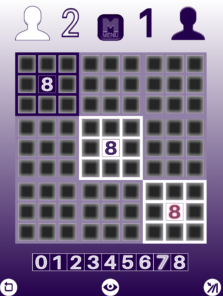
\includegraphics[scale=0.5]{img/tutorial_1.png}
\end{center}

\pagebreak
\begin{itemize}
    \item Players receive points equal to the number in the region where the number is placed. These points 
    are known as \textbf{Power}.
\end{itemize}
\begin{center}
    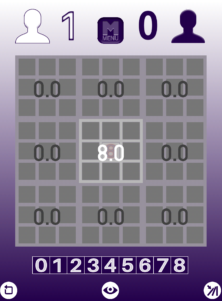
\includegraphics[scale=0.5]{img/tutorial_2.png}
\end{center}

\begin{itemize}
    \item If a number borders other regions, horizontally, vertically or diagonally, the player receives 
    1/2 points in those border regions.  These points are known as \textbf{Influence}.
\end{itemize}
\begin{center}
    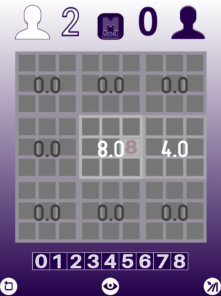
\includegraphics[scale=0.5]{img/tutorial_3.png}
\end{center}

\begin{itemize}
    \item Placement conforms to the rules of Sudoku, so a number may only be placed once in a region, row or 
    column. (Broken Sudoku will occur.)
    \item When all numbers that can be placed have been placed, the gameboard is resolved. \textbf{Resolution} 
    determines the outcome.
\end{itemize}

\pagebreak
\subsubsection{Resolution Phase}

\begin{itemize}
    \item Regions are resolved in order of the greatest disparity. These are the regions with greatest point 
    difference between players.
\end{itemize}
\begin{center}
    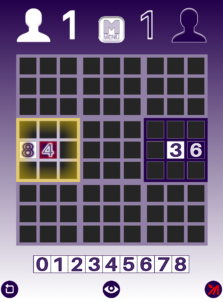
\includegraphics[scale=0.5]{img/tutorial_4.png}
\end{center}

\begin{itemize}
    \item When a region is resolved, it is awarded to the player with the most points in the region, known as the dominant player.
    \item All opposing numbers in that region defect, flipping to the dominant player. This player is now said to have control.
\end{itemize}
\begin{center}
    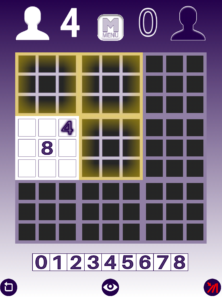
\includegraphics[scale=0.5]{img/tutorial_5.png}
\end{center}

\begin{itemize}
    \item If these numbers border other regions, they switch their \textbf{Influence} points. (This can shift the balance of power, 
    affecting the outcome of the game!)
\end{itemize}
\begin{center}
    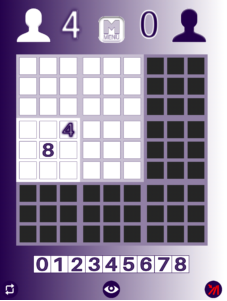
\includegraphics[scale=0.5]{img/tutorial_6.png}
\end{center}

\begin{itemize}
    \item When all regions that can be resolved, have been resolved, the player controlling the most regions wins.
    \item Strength of victory is measured by the ratio of controlled regions between players, such as 5/4, 4/5, 4/4, 9/0, 0/9,\ldots
\end{itemize}

\paragraph{}
The official rules can be consulted in the address: http://mbranegame.com/rules-of-m \cite{Rules}.

%%%%%%%%%%%%%%%%%%%%%%%%%%
\pagebreak
\section{Game Logic}

\subsection{Game state representation} 
Although the user can only be able to see one board at a time, in a any phase of the game, there are actually three
boards represented in the game’s data structures. There’s a board predicate that represents the game board itself, a
list of 9 lists each representing a line of the board. This is the board used to print the state of the game. There’s 
also a \textbf{board\_blocks} predicate. This predicate is also a list of 9 lists, each one representing a 3 by 3 block of the 
board, this is used to facilitate calculations involving power in each block and influence in adjacent blocks caused 
by the placement of a number in the edge of a block. Finally we have a \textbf{board\_influence} list that stores the values of 
power (and spread influence) in each block of the board.  When a player adds a number to cell, all the boards are 
updated accordingly.


\subsection{Board viewing} 
Before each move, the board is displayed on the screen. To display the board we use the predicate \textit{display\_game(+Board, +Player1, +Player2)}. This predicate first displays the players' names and then uses \textit{display\_board(+Board)} to display the board itself. 
The board is displayed line by line with a series of dividers. Although for game logic the values of the board can be positive or negative, the board is printed with only positive numbers.

\subsection{List valid plays} 
As per requested, we developed a predicate that returns a list of all possible moves. This predicate is \textit{valid\_moves(+Board, -R)}. The first argument of the predicate is a list with the board of lines and board of blocks.
This predicate works by first finding a list of all empty cells with \textit{check\_all(+Board, -List),}. Then it tests all possible values in those cells with \textit{test_all(+List, +Board, +Result)}.

\subsection{Play execution} 
Each player can make a move per turn \textit{player\_turn(+Board, +Player, -NewBoard)}. In this turn predicate, the program asks the player what he wants to play with \textit{get_move(-X, -Y, -V)} then the program tries that move with \textit{move(+Move, +Board, -NewBoard)}.
If the move is invalid the program repeats the previous action, otherwise, it returns a new board with the new piece.

\paragraph{}
The number placing rules are the ones of Sudoku, so the player can only place a number if that same number is not present
in either the column, row or 3x3 section of the square the player wants to place it. If these conditions are met, 
the number is able to be placed.

\subsection{Game finalization} 
For the end of game we need to verify if there are any possible moves left. This is done by predicate \textit{game\_over(+Board, -Winner)}. If there are any moves left, it fails and the game continues.
Otherwise it will find out who won the game. This is done by verifying which player controls the most blocks in the predicate \textit{get\_winner(+Board, -Winner)}.

% TODO complete
\subsection{Board evaluation}
Avaliação do estado do jogo, que permitirá comparar a aplicação das diversas jogadas disponíveis. O predicado deve chamar-se \textit{value(+Board, +Player, -Value)}.

% TODO complete
\subsection{Plays of the computer} 
Escolha da jogada a efetuar pelo computador, dependendo do nível de dificuldade. O predicado deve chamar-se \textit{choose\_move(+Board, +Level, -Move)}.



%%%%%%%%%%%%%%%%%%%%%%%%%%
\pagebreak
% TODO complete
\section{Conclusions}
With this work we have developed our way of thinking in a new way. Although Prolog can be compared to other programming languages, it is unique in the way it works.
The biggest problem we found was trying to make use of dynamic predicates to create a sort of global board. After testing a lot we decided to give up on the idea.
In terms of the game mechanics, there are a lot of verifications 


\clearpage
%\addcontentsline{toc}{section}{Bibliografia}
\renewcommand\refname{Apendix}
\bibliographystyle{apalike}
\bibliography{myrefs}

\newpage
\appendix
% \section{Nome do Anexo}
% Outros elementos úteis que não sejam essenciais ao relatório.

\end{document}
